%%%% Document setup
\documentclass[a4paper,landscape,title page]{article}
\setlength{\oddsidemargin}{-0.65in}	% default=0in
\setlength{\textwidth}{11in}		% default=9in
\setlength{\textheight}{6.85in}		% default=5.15in
\setlength{\topmargin}{-1.0in}		% default=0.20in
\setlength{\headsep}{0.35in}		% default=0.35in
\setlength{\parskip}{1.2ex}
\setlength{\parindent}{0mm}

%%%% Use packages
\usepackage{times}
\usepackage{tikz,pgf}
\usetikzlibrary{arrows,automata,trees,plotmarks,calc}


%%%%
\title{Goal-Plan hierarchy for test \textit{testfr02}}
\author{
Dhirendra Singh\\
dhirendra.singh@rmit.edu.au}
\begin{document}
\maketitle

\begin{figure*}[t]
\begin{center}

\begin{tikzpicture}[scale=1.1,level distance=1.4cm]
\tikzstyle{txt}=[scale=1.1]
\tikzstyle{planbox}=[scale=1.1,draw,minimum height=0.7cm,minimum width=1.1cm]
\tikzstyle{goalbox}=[scale=1.1,draw,rounded corners,minimum height=0.7cm,minimum width=1.1cm]
\tikzstyle{level 1}=[sibling distance=4.0cm] 
\tikzstyle{level 2}=[sibling distance=6.0cm] 
\tikzstyle{level 3}=[sibling distance=3.0cm]
\tikzstyle{level 4}=[sibling distance=3.0cm]
\tikzstyle{level 5}=[sibling distance=1.5cm]
\tikzstyle{level 6}=[sibling distance=3.0cm]
\tikzstyle{level 7}=[sibling distance=1.5cm]

\node[goalbox,yshift=1cm,solid] (T) {$G$}
	child[solid] {node[planbox] (P1) {$P_1$}
		child {node[goalbox] {$G_{a}$}
			child {node[planbox] {$P_{a1}$}
				child {node[goalbox] {$G_{aa}$}
					child {node[planbox] {$P_{aa1}$}
						child {node[goalbox] {$G_{aaa}$}
							child {node[planbox] {$P_{aaa1}$} node[txt,below=0.3cm] {$\surd$}}
							child {node[planbox] {$P_{aaa*}$} node[txt,below=0.3cm] {$\times$}
								edge from parent node[txt,right,near start] {$\times 2$}
							}
							edge from parent node[txt,right] {$\times 2$}
						}
					}
					child {node[planbox] {$P_{aa*}$} node[txt,below=0.3cm] {$\times$}
						edge from parent node[txt,right,near start] {$\times 3$}
					}
				}
				child {node[goalbox] {$G_{ab}$}
					child {node[planbox] {$P_{ab1}$} node[txt,below=0.3cm] {$\surd$}}
					child {node[planbox] {$P_{ab*}$} node[txt,below=0.3cm] {$\times$}
						edge from parent node[txt,right,near start] {$\times 2$}
					}
				}
			}
			child {node[planbox] {$P_{a*}$} node[txt,below=0.3cm] {$\times$}
				edge from parent node[txt,right,near start] {$\times 3$}
			}
		}
		child {node[goalbox] {$G_{b}$}
			child {node[planbox] {$P_{b1}$}
				child {node[goalbox] {$G_{ba}$}
					child {node[planbox] {$P_{ba1}$}
						child {node[goalbox] {$G_{baa}$}
							child {node[planbox] {$P_{baa1}$} node[txt,below=0.3cm] {$\surd$}}
							child {node[planbox] {$P_{baa*}$} node[txt,below=0.3cm] {$\times$}
								edge from parent node[txt,right,near start] {$\times 2$}
							}
							edge from parent node[txt,right] {$\times 2$}
						}
					}
					child {node[planbox] {$P_{ba*}$} node[txt,below=0.3cm] {$\times$}
						edge from parent node[txt,right,near start] {$\times 3$}
					}
				}
				child {node[goalbox] {$G_{bb}$}
					child {node[planbox] {$P_{bb1}$} node[txt,below=0.3cm] {$\surd$}}
					child {node[planbox] {$P_{bb*}$} node[txt,below=0.3cm] {$\times$}
						edge from parent node[txt,right,near start] {$\times 2$}
					}
				}
			}
			child {node[planbox] {$P_{b*}$} node[txt,below=0.3cm] {$\times$}
				edge from parent node[txt,right,near start] {$\times 3$}
			}
		}
		child {node[goalbox] {$G_{c}$}
			child {node[planbox] {$P_{c1}$}
				child {node[goalbox] {$G_{ca}$}
					child {node[planbox] {$P_{ca1}$}
						child {node[goalbox] {$G_{caa}$}
							child {node[planbox] {$P_{caa1}$} node[txt,below=0.3cm] {$\surd$}}
							child {node[planbox] {$P_{caa*}$} node[txt,below=0.3cm] {$\times$}
								edge from parent node[txt,right,near start] {$\times 2$}
							}
							edge from parent node[txt,right] {$\times 2$}
						}
					}
					child {node[planbox] {$P_{ca*}$} node[txt,below=0.3cm] {$\times$}
						edge from parent node[txt,right,near start] {$\times 3$}
					}
				}
				child {node[goalbox] {$G_{cb}$}
					child {node[planbox] {$P_{cb1}$} node[txt,below=0.3cm] {$\surd$}}
					child {node[planbox] {$P_{cb*}$} node[txt,below=0.3cm] {$\times$}
						edge from parent node[txt,right,near start] {$\times 2$}
					}
				}
			}
			child {node[planbox] {$P_{c*}$} node[txt,below=0.3cm] {$\times$}
				edge from parent node[txt,right,near start] {$\times 3$}
			}
		}
	}
;

\end{tikzpicture}

\vskip 1.5cm
\caption{The hierarchy has 4 top level plans $P_1 \ldots P_4$ and the total number of worlds is $2^5$. Only $P_1$ has the solutions, $P_2 \ldots P_4$ are all single action plans that always fail. Successful execution trace is of length $9$ distributed between goals $G_a \ldots G_c$. The aim is to compare how many actions it takes on average for the top level goal $G$ to succeed --- with and without failure recovery. The intuition is that failure recovery should help learn $G$ faster. For instance, say we have learnt to achieve $G_a$ and $G_b$. Then to learn $G_c$ we must first perform $G_a$, then $G_b$ and then try different options as we acquire experience in $G_c$. If we were to re-post $G$ after each failure then for each unsuccessful choice in $G_c$ we have to do a lot of re-work (i.e. achieve $G_a$ and $G_b$ again) before we can try something else. With failure recovery enabled however, when learning $G_c$ we only perform $G_a$ and $G_b$ once and then exhaust all options for $G_c$ in a single try. However, this assumes that failures do not (generally) change the world in such a way that alternatives tried with failure recovery will never succeed. If that were the case then failure recovery would perform worse than reposting.}
\end{center}
\end{figure*}

\end{document}
%%%%